\documentclass{estilo}
\usepackage[spanish]{babel}
\usepackage{graphicx}
\usepackage{float}
\usepackage{amsmath}        % para los vectores columnas
\usepackage{amsfonts}       % para las negrita de pizarra
\usepackage{amssymb}        % para simbolos matematicos
\usepackage{hyperref}       % para utilizar referencias
\usepackage{multirow}       % para las tablas
\usepackage{dsfont}
\usepackage{listings}
\usepackage{xcolor}
\definecolor{codegreen}{rgb}{0,0.6,0}
\definecolor{codegray}{rgb}{0.5,0.5,0.5}
\definecolor{codepurple}{rgb}{0.58,0,0.82}
\definecolor{backcolour}{rgb}{0.95,0.95,0.92}
\lstdefinestyle{mystyle}{
    backgroundcolor=\color{backcolour},   
    commentstyle=\color{codegreen},
    keywordstyle=\color{magenta},
    numberstyle=\tiny\color{codegray},
    stringstyle=\color{codepurple},
    basicstyle=\ttfamily\footnotesize,
    breakatwhitespace=false,         
    breaklines=true,                 
    captionpos=b,                    
    keepspaces=true,                 
    numbers=left,                    
    numbersep=5pt,                  
    showspaces=false,                
    showstringspaces=false,
    showtabs=false,                  
    tabsize=2
}
\lstset{style=mystyle}

\usepackage{enumitem,multicol,setspace}
\newcounter{subenum}[enumi] % para las multicolumnas
\renewcommand{\thesubenum}{\arabic{subenum}}
\usepackage[nomessages]{fp}
\FPeval\thecolwidth{round(1/4:4)}% Specify number of columns -> column width
\newcommand{\newitem}[1]{%
  \refstepcounter{subenum}%
  \parbox{\dimexpr\thecolwidth\linewidth-.5\columnsep}{%
    \makebox[\labelwidth][r]{(\thesubenum)\hspace*{\labelsep}}%
    #1}\hfill%
}

\usepackage{scalerel,stackengine} % para el sombrero
\stackMath
\newcommand\rhat[1]{%
\savestack{\tmpbox}{\stretchto{%
  \scaleto{%
    \scalerel*[\widthof{\ensuremath{#1}}]{\kern-.6pt\bigwedge\kern-.6pt}%
    {\rule[-\textheight/2]{1ex}{\textheight}}%WIDTH-LIMITED BIG WEDGE
  }{\textheight}% 
}{0.5ex}}%
\stackon[1pt]{#1}{\tmpbox}%
}
\parskip 1ex

\usepackage{mathtools}      % floor y ceil
\DeclarePairedDelimiter\ceil{\lceil}{\rceil}
\DeclarePairedDelimiter\floor{\lfloor}{\rfloor} 

\usepackage[style=authoryear-comp]{biblatex}


\begin{document}
\maketitle

\justifying{
}

% \newpage
% \input{tex/consideraciones}
\newpage

\section{Análisis del problema}

El problema consiste en determinar la máxima cantidad de ganancia que se puede obtener de una secuencia de entrenamientos, manteniendo en consideración que si se entrena se tendrá una energía menor o igual el día siguiente y que la misma se restablece completamente si se descansa un día. Como datos de entrada tenemos una secuencia de energía disponible por día según cuando fue el último descanso, denotada como $s_1, s_2, ..., s_n$, y el esfuerzo/ganancia potencial máximo que se puede obtener por cada día $e_i$.

\section{Algoritmo Greedy}

No es posible llegar a una solución óptima a través de un algoritmo Greedy. Esto podemos verlo planteando un simple contraejemplo: si comparamos la ganancia de entrenar los primeros dos días o descansar el primero y entrenar el segundo, podríamos pensar que conviene descansar si el segundo día obtenemos una ganancia mayor. Sin embargo, estaríamos ignorando el hecho de que el tercer día podría estar dando una mejor ganancia que el segundo y sea más conveniente entrenar el primer día y el tercero.

\section{Ecuación de recurrencia}
Para abordar este problema necesitamos formular una ecuación recurrente que nos permita conocer la ganancia que obtendríamos si entrenáramos un día $i$ con $d$ días de descanso hasta el fin del entrenamiento. De esta forma, la ecuación seria:
\[f(i, d) = \max\left\{
\begin{array}{ll}
f(i+1, d+1) + g_i & \text{si entreno el día } i \\
f(i+1, 0) & \text{si descanso el día } i
\end{array}
\right.
\]

Donde:
\begin{itemize}
    \item $g_i$ es la ganancia del día $i$ habiendo descansado $d+1$ días.
    \item $f(i+1, d+1) + g_i $ representa entrenar el día $i$, lo que nos proporciona la ganancia potencial del día más la máxima ganancia acumulada desde el día siguiente $i+1$ hasta el último día con $d$ días desde el último descanso. 
    \item $f(i+1, 0)$ representa tomar un descanso el día $i$, lo que nos reinicia el contador de días desde el último descanso ($d$ se establece en 0) y calcula la máxima ganancia acumulada desde el día siguiente $i+1$ hasta el último día.
\end{itemize}

% Para abordar este problema a través de la programación dinámica, podemos plantear una ecuación de recurrencia que nos permita calcular la máxima ganancia acumulada hasta el día $i$, considerando el número de días desde el último descanso, denotado como $d$. Utilizando una matriz de memorización denominada $M$ podemos denotar $M[i][d]$ como la máxima ganancia acumulada hasta el día $i$ con $d$ días desde el último descanso. La ecuación de recurrencia sería:

% \[M[i][d] = \max\left\{
% \begin{array}{ll}
% M[i-1][d+1] + e_i & \text{si entreno el día } i \\
% M[i-1][0] & \text{si descanso el día } i
% \end{array}
% \right.
% \]

% Donde:
% \begin{itemize}
%     \item $e_i$ es la ganancia potencial propia del día $i$.
%     \item $M[i-1][d+1] + e_i$ representa entrenar el día $i$, lo que nos proporciona la ganancia potencial del día más la máxima ganancia acumulada hasta el día $i-1$ con $d+1$ días desde el último descanso. 
%     \item $M[i-1][0]$ representa tomar un descanso el día $i$, lo que nos reinicia el contador de días desde el último descanso ($d$ se establece en 0).
% \end{itemize}

\newpage

\section{El algoritmo}

\subsection{La memorización}
Luego de obtener la ecuación de recurrencia, podemos plantear un algoritmo recurrente para resolver el problema. Utilizamos este algoritmo para resolver los tests y verificar su funcionamiento, sin embargo, notamos que aún con pocos elementos se volvía muy lento. Esto se debe a que vuelve a calcular las ganancias óptimas múltiple cantidad de veces.

Obtuvimos mejoras en el rendimiento cuando incorporamos una matriz para guardar los resultados y pasamos de tener un tiempo de ejecución exponencial a uno lineal.

Sin embargo, seguimos teniendo problemas con pruebas de volumen porque el programa superaba el límite de llamadas recursivas y finalizaba abruptamente, por lo cuál, cambiamos el enfoque del algoritmo recursivo Top-Down a un algoritmo iterativo Bottom-Up.

\subsection{Construir la matriz de óptimos}
La primera etapa del algoritmo consiste en llenar una matriz de memorización $M$, que se utiliza para registrar la máxima ganancia acumulada hasta el día $i$ considerando el número de días desde el último descanso, denotado como $d$.

Para ello, comenzamos iterando sobre los días de entrenamiento desde el inicio hasta el último día.
En cada iteración, calculamos la ganancia potencial del día actual $e_i$ y la almacenamos en la matriz $M[i][d]$. Esto representa la máxima ganancia que podríamos obtener si entrenáramos el día $i$ con $d$ días desde el último descanso. Luego utilizamos la ecuación de recurrencia mencionada en el informe: $M[i][d] = \max{M[i+1][d+1] + e_i, M[i+1][0]}$ para calcular el valor óptimo. Aquí, comparamos dos opciones: entrenar el día $i$ o tomar un descanso, y elegimos la que maximice la ganancia acumulada.

Este proceso de llenado de la matriz de memorización se realiza en un bucle anidado, que recorre todos los días y los posibles valores de días desde el último descanso. Debido a esto, la complejidad de esta etapa es $O(n^2)$, donde $n$ es la cantidad de días en la secuencia de entrenamientos.

\begin{lstlisting}[language=Python]
def mejor_ganancia_iterativo(ganancia_por_dia, energia_por_dia) -> Tuple[int, List[int]]:
    cant_dias = len(ganancia_por_dia)

    M = [[0 for _ in range(cant_dias+1)] for _ in range(cant_dias+1)]
    
    for dia_a_analizar in range(cant_dias):
        for dias_desde_descanso in range(dia_a_analizar + 1):
            M[dia_a_analizar][dias_desde_descanso] = _ganancia_del_dia(dia_a_analizar, dias_desde_descanso, ganancia_por_dia, energia_por_dia)
    
    for dia_a_analizar in range(cant_d  ias-1, -1, -1):
        for dias_desde_descanso in range(dia_a_analizar + 1):
            ganancia_si_descanso = M[dia_a_analizar+1][0]
            ganancia_si_entreno = M[dia_a_analizar][dias_desde_descanso] + M[dia_a_analizar+1][dias_desde_descanso+1]
            M[dia_a_analizar][dias_desde_descanso] = max(ganancia_si_descanso, ganancia_si_entreno)
    
    ganancia= M[0][0]
    plan = _reconstruir_plan_de_entrenamiento_desde_memo(M, ganancia_por_dia, energia_por_dia)
    return ganancia, plan
\end{lstlisting}

\newpage
\subsection{Reconstruir el plan de entrenamiento óptimo}
La segunda etapa del algoritmo consiste en reconstruir el plan de entrenamiento óptimo, es decir, determinar qué días debemos entrenar y cuáles debemos tomar un descanso para obtener la máxima ganancia.

Para esto comenzamos desde el primer día y avanzamos hacia el último día. Evaluando, en cada paso, si es óptimo entrenar en el día actual o tomar un descanso utilizando la información almacenada en la matriz de memorización $M$ para tomar esta decisión. Si es óptimo entrenar, agregamos el día actual al plan de entrenamiento. Si, en cambio, es óptimo descansar, reiniciamos el contador de días desde el último descanso.
Este proceso se realiza en un bucle que recorre todos los días de la secuencia de entrenamientos, por lo que su complejidad es $O(n)$.

\begin{lstlisting}[language=Python]
def _reconstruir_plan_de_entrenamiento_desde_memo(M, ganancia_por_dia, energia_por_dia) -> List[int]:
    cant_dias = len(ganancia_por_dia)
    plan = []

    dias_desde_descanso = 0
    for dia_a_analizar in range(cant_dias):
        # el ultimo dia siempre entreno
        if dia_a_analizar == cant_dias - 1:
            plan.append(ENTRENO)
            dias_desde_descanso += 1
            continue

        ganancia_optima = M[dia_a_analizar][dias_desde_descanso]
        ganancia_del_dia = _ganancia_del_dia(dia_a_analizar, dias_desde_descanso, ganancia_por_dia, energia_por_dia)
        ganancia_si_entreno = M[dia_a_analizar+1][dias_desde_descanso+1]

        if ganancia_optima == ganancia_del_dia + ganancia_si_entreno:
            plan.append(ENTRENO)
            dias_desde_descanso += 1
            continue

        plan.append(DESCANSO)
        dias_desde_descanso = 0

    return plan

\end{lstlisting}

\section{Complejidad computacional del Algoritmo}

Podemos analizar la complejidad del algoritmo en dos fases (como ya las hemos mencionado anteriormente): \textbf{La construcción de la matriz de óptimos y la posterior reconstrucción del plan de entrenamiento}. 

En la primera fase, la construcción de la matriz de tamaño $n \times n$, observamos la utilización de dos bucles anidados. El bucle externo recorre los días de entrenamiento desde el inicio hasta el último día, mientras que el bucle interno itera sobre los días desde el último descanso hasta el valor actual del bucle externo. Dentro de este bucle, se realizan operaciones de asignación de valores en la matriz, lo que implica tiempo constante por cada iteración. Como resultado de esta etapa obtenemos una complejidad cuadrática, es decir, $O(n^2)$.

En la segunda fase, que es la reconstrucción del plan de entrenamiento óptimo, se realiza un recorrido lineal de los días de 0 a $n$, con operaciones dentro del bucle que son de tiempo constante. Por lo tanto, la complejidad de esta etapa es lineal, $O(n)$. 

Sin embargo, la complejidad total del algoritmo está dominada por la fase de llenado de la matriz de memorización. Por lo tanto, \textbf{la complejidad termina siendo $O(n^2)$}.

\newpage

\section{Mediciones}
\subsection{Metodología}

Para realizar las mediciones utilizamos el archivo \texttt{tiempos\_ejecución\_final.ipynb}, donde procedimos a calcular el tiempo que toman nuestros algoritmos en hacer el análisis en base a la cantidad de días correspondientes utilizando slices del archivo \texttt{5000.txt} para los datos de muestreo. 

Esto se realizo a través de la siguiente función:
\begin{lstlisting}[language=Python]
# medir
from timeit import timeit

# graficar
import pandas as pd

# tp2
from tp2.archivos import leer_archivo
from tp2.entrenamiento import *

ganancia_por_dia, energia_por_dia = leer_archivo("../examples/5000.txt")

def medir_mejor_ganancia(cant_dias, metodo):
    print(f"Midiendo para {cant_dias} dias")
    iteraciones = 3
    _ganancia_por_dia = ganancia_por_dia[:cant_dias]
    tiempo_ejecucion = timeit(lambda: metodo(_ganancia_por_dia, energia_por_dia), number=iteraciones) / iteraciones
    return tiempo_ejecucion * 1000
\end{lstlisting}

Que nos permitió realizar los gráficos utilizando la librería pandas en base al siguiente template:
\begin{lstlisting}[language=Python]
mediciones = 10
step = 1
cant_dias = [i + step for i in range(0, mediciones * step, step)]

k = 3.557503204650629e-04

df = pd.DataFrame({
    "Recursivamente sin memorizacion": [medir_mejor_ganancia(dias, mejor_ganancia_recursivo) for dias in cant_dias],
    "Recursivamente con memorizacion": [medir_mejor_ganancia(dias, mejor_ganancia_recursivo_con_memoria) for dias in cant_dias],
    "Iterativamente con memorizacion": [medir_mejor_ganancia(dias, mejor_ganancia_iterativo) for dias in cant_dias],
    "O(k * n^2) con k = 3.5575e-04": [k * dias ** 2 for dias in cant_dias]
    }, index=cant_dias)

print(df.shape)

plot = df.plot.line(
    title="Tiempo de ejecucion segun cantidad de dias",
    xlabel="Cantidad de dias",
    ylabel="Tiempo de ejecucion (Ms)",
)
\end{lstlisting}
Este template nos permitió ir cambiando que implementaciones, Ks y datasets utilizábamos en cada gráfico rápida y concisamente.
\newpage
\subsection{Resultados}

Para corroborar nuestro análisis teórico de la complejidad graficamos, siguiendo los procesos antes descriptos, los tiempos de ejecución de los distintos algoritmos que fuimos implementando contra la curva $O(n^2)$:

\begin{center}
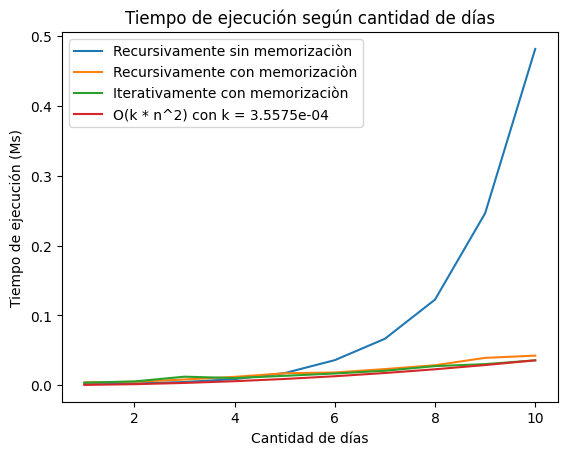
\includegraphics[width=0.7\textwidth]{img/Results.png}
\end{center}
Como se puede ver en el gráfico anterior la curva de la solución sin uso de memorización  hace que las curvas $O(n^2)$ parezcan lineales ya que esta tiene una complejidad de $O(n^n)$
\begin{center}
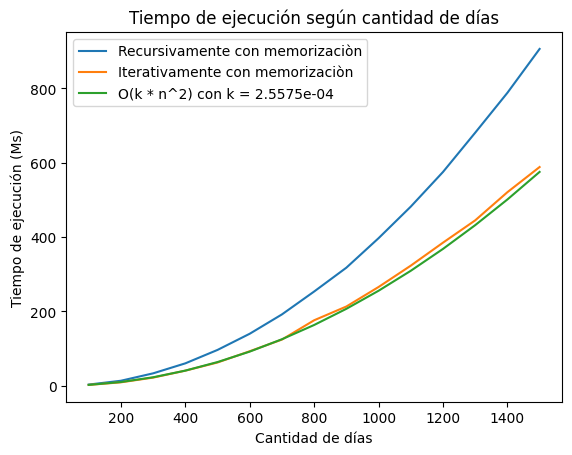
\includegraphics[width=0.7\textwidth]{img/Results2.png}
\end{center}
Con este gráfico podemos ver que hay una marcada diferencia entre los tiempos de ejecución de la solución recursiva contra la iterativa a pesar de que ambos cuentan con la misma complejidad algorítmica.
\begin{center}
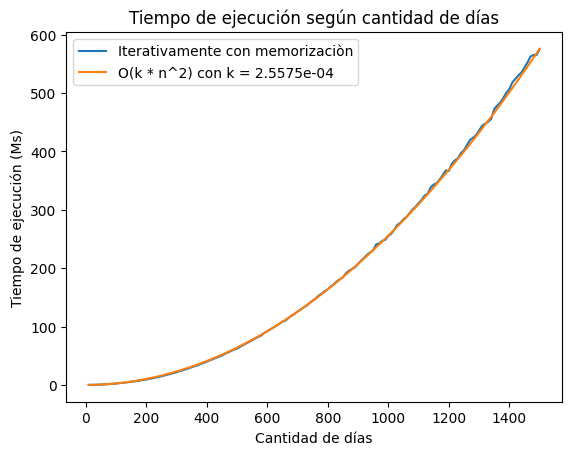
\includegraphics[width=0.7\textwidth]{img/Results3.png}
\end{center}
Finalmente, sumando un poco de resolución al dataset del gráfico, podemos ver como la solución iterativa sigue casi perfectamente a la curva $O(n^2)$

\section{Conclusiones}
Podemos concluir que la solución mediante Programación Dinámica nos permitió encontrar una solución óptima evitando explorar un espacio exponencial de soluciones como se haría a través de la alternativa de resolverlo por fuerza bruta, por lo cual, gracias a esta metodología pudimos reducir la complejidad temporal de nuestro algoritmo significativamente. También corroboramos que los tiempos de ejecución se comportaban de la manera esperada según la complejidad que habíamos calculado ($O(n ^ 2)$) para resolver este problema y encontramos diferencias en los tiempos de ejecución entre las implementaciones iterativas y recursivas del algoritmo con memorización. 

El algoritmo recursivo termina siendo más lento y consume mucho más memoria debido a las múltiples llamadas recursivas que hace y que mantiene en el stack durante su ejecución. Además, la implementación recursiva puede llevar a problemas de stack thrashing con datasets mas grandes. En base a esto identificamos que tenemos que cambiar el enfoque de la solución de subproblemas de Top-Down a Bottom-Up.

Finalmente:
\begin{center}

\includegraphics[width=0.7\textwidth]{img/Scaloni.png}
\end{center}

\end{document}

\documentclass{article}
\usepackage{amsmath}
